% Options for packages loaded elsewhere
\PassOptionsToPackage{unicode}{hyperref}
\PassOptionsToPackage{hyphens}{url}
%
\documentclass[
  man,floatsintext]{apa7}
\usepackage{amsmath,amssymb}
\usepackage{iftex}
\ifPDFTeX
  \usepackage[T1]{fontenc}
  \usepackage[utf8]{inputenc}
  \usepackage{textcomp} % provide euro and other symbols
\else % if luatex or xetex
  \usepackage{unicode-math} % this also loads fontspec
  \defaultfontfeatures{Scale=MatchLowercase}
  \defaultfontfeatures[\rmfamily]{Ligatures=TeX,Scale=1}
\fi
\usepackage{lmodern}
\ifPDFTeX\else
  % xetex/luatex font selection
\fi
% Use upquote if available, for straight quotes in verbatim environments
\IfFileExists{upquote.sty}{\usepackage{upquote}}{}
\IfFileExists{microtype.sty}{% use microtype if available
  \usepackage[]{microtype}
  \UseMicrotypeSet[protrusion]{basicmath} % disable protrusion for tt fonts
}{}
\makeatletter
\@ifundefined{KOMAClassName}{% if non-KOMA class
  \IfFileExists{parskip.sty}{%
    \usepackage{parskip}
  }{% else
    \setlength{\parindent}{0pt}
    \setlength{\parskip}{6pt plus 2pt minus 1pt}}
}{% if KOMA class
  \KOMAoptions{parskip=half}}
\makeatother
\usepackage{xcolor}
\usepackage{graphicx}
\makeatletter
\def\maxwidth{\ifdim\Gin@nat@width>\linewidth\linewidth\else\Gin@nat@width\fi}
\def\maxheight{\ifdim\Gin@nat@height>\textheight\textheight\else\Gin@nat@height\fi}
\makeatother
% Scale images if necessary, so that they will not overflow the page
% margins by default, and it is still possible to overwrite the defaults
% using explicit options in \includegraphics[width, height, ...]{}
\setkeys{Gin}{width=\maxwidth,height=\maxheight,keepaspectratio}
% Set default figure placement to htbp
\makeatletter
\def\fps@figure{htbp}
\makeatother
\setlength{\emergencystretch}{3em} % prevent overfull lines
\providecommand{\tightlist}{%
  \setlength{\itemsep}{0pt}\setlength{\parskip}{0pt}}
\setcounter{secnumdepth}{-\maxdimen} % remove section numbering
% Make \paragraph and \subparagraph free-standing
\ifx\paragraph\undefined\else
  \let\oldparagraph\paragraph
  \renewcommand{\paragraph}[1]{\oldparagraph{#1}\mbox{}}
\fi
\ifx\subparagraph\undefined\else
  \let\oldsubparagraph\subparagraph
  \renewcommand{\subparagraph}[1]{\oldsubparagraph{#1}\mbox{}}
\fi
\newlength{\cslhangindent}
\setlength{\cslhangindent}{1.5em}
\newlength{\csllabelwidth}
\setlength{\csllabelwidth}{3em}
\newlength{\cslentryspacingunit} % times entry-spacing
\setlength{\cslentryspacingunit}{\parskip}
\newenvironment{CSLReferences}[2] % #1 hanging-ident, #2 entry spacing
 {% don't indent paragraphs
  \setlength{\parindent}{0pt}
  % turn on hanging indent if param 1 is 1
  \ifodd #1
  \let\oldpar\par
  \def\par{\hangindent=\cslhangindent\oldpar}
  \fi
  % set entry spacing
  \setlength{\parskip}{#2\cslentryspacingunit}
 }%
 {}
\usepackage{calc}
\newcommand{\CSLBlock}[1]{#1\hfill\break}
\newcommand{\CSLLeftMargin}[1]{\parbox[t]{\csllabelwidth}{#1}}
\newcommand{\CSLRightInline}[1]{\parbox[t]{\linewidth - \csllabelwidth}{#1}\break}
\newcommand{\CSLIndent}[1]{\hspace{\cslhangindent}#1}
\ifLuaTeX
\usepackage[bidi=basic]{babel}
\else
\usepackage[bidi=default]{babel}
\fi
\babelprovide[main,import]{english}
% get rid of language-specific shorthands (see #6817):
\let\LanguageShortHands\languageshorthands
\def\languageshorthands#1{}
% Manuscript styling
\usepackage{upgreek}
\captionsetup{font=singlespacing,justification=justified}

% Table formatting
\usepackage{longtable}
\usepackage{lscape}
% \usepackage[counterclockwise]{rotating}   % Landscape page setup for large tables
\usepackage{multirow}		% Table styling
\usepackage{tabularx}		% Control Column width
\usepackage[flushleft]{threeparttable}	% Allows for three part tables with a specified notes section
\usepackage{threeparttablex}            % Lets threeparttable work with longtable

% Create new environments so endfloat can handle them
% \newenvironment{ltable}
%   {\begin{landscape}\centering\begin{threeparttable}}
%   {\end{threeparttable}\end{landscape}}
\newenvironment{lltable}{\begin{landscape}\centering\begin{ThreePartTable}}{\end{ThreePartTable}\end{landscape}}

% Enables adjusting longtable caption width to table width
% Solution found at http://golatex.de/longtable-mit-caption-so-breit-wie-die-tabelle-t15767.html
\makeatletter
\newcommand\LastLTentrywidth{1em}
\newlength\longtablewidth
\setlength{\longtablewidth}{1in}
\newcommand{\getlongtablewidth}{\begingroup \ifcsname LT@\roman{LT@tables}\endcsname \global\longtablewidth=0pt \renewcommand{\LT@entry}[2]{\global\advance\longtablewidth by ##2\relax\gdef\LastLTentrywidth{##2}}\@nameuse{LT@\roman{LT@tables}} \fi \endgroup}

% \setlength{\parindent}{0.5in}
% \setlength{\parskip}{0pt plus 0pt minus 0pt}

% Overwrite redefinition of paragraph and subparagraph by the default LaTeX template
% See https://github.com/crsh/papaja/issues/292
\makeatletter
\renewcommand{\paragraph}{\@startsection{paragraph}{4}{\parindent}%
  {0\baselineskip \@plus 0.2ex \@minus 0.2ex}%
  {-1em}%
  {\normalfont\normalsize\bfseries\itshape\typesectitle}}

\renewcommand{\subparagraph}[1]{\@startsection{subparagraph}{5}{1em}%
  {0\baselineskip \@plus 0.2ex \@minus 0.2ex}%
  {-\z@\relax}%
  {\normalfont\normalsize\itshape\hspace{\parindent}{#1}\textit{\addperi}}{\relax}}
\makeatother

\makeatletter
\usepackage{etoolbox}
\patchcmd{\maketitle}
  {\section{\normalfont\normalsize\abstractname}}
  {\section*{\normalfont\normalsize\abstractname}}
  {}{\typeout{Failed to patch abstract.}}
\patchcmd{\maketitle}
  {\section{\protect\normalfont{\@title}}}
  {\section*{\protect\normalfont{\@title}}}
  {}{\typeout{Failed to patch title.}}
\makeatother

\usepackage{xpatch}
\makeatletter
\xapptocmd\appendix
  {\xapptocmd\section
    {\addcontentsline{toc}{section}{\appendixname\ifoneappendix\else~\theappendix\fi\\: #1}}
    {}{\InnerPatchFailed}%
  }
{}{\PatchFailed}
\keywords{keywords\newline\indent Word count: X}
\usepackage{csquotes}
\makeatletter
\renewcommand{\paragraph}{\@startsection{paragraph}{4}{\parindent}%
  {0\baselineskip \@plus 0.2ex \@minus 0.2ex}%
  {-1em}%
  {\normalfont\normalsize\bfseries\typesectitle}}

\renewcommand{\subparagraph}[1]{\@startsection{subparagraph}{5}{1em}%
  {0\baselineskip \@plus 0.2ex \@minus 0.2ex}%
  {-\z@\relax}%
  {\normalfont\normalsize\bfseries\itshape\hspace{\parindent}{#1}\textit{\addperi}}{\relax}}
\makeatother

\ifLuaTeX
  \usepackage{selnolig}  % disable illegal ligatures
\fi
\IfFileExists{bookmark.sty}{\usepackage{bookmark}}{\usepackage{hyperref}}
\IfFileExists{xurl.sty}{\usepackage{xurl}}{} % add URL line breaks if available
\urlstyle{same}
\hypersetup{
  pdftitle={How Foreign Language Impacts Moral Decision Making},
  pdfauthor={Lindsey King1},
  pdflang={en-EN},
  pdfkeywords={keywords},
  hidelinks,
  pdfcreator={LaTeX via pandoc}}

\title{How Foreign Language Impacts Moral Decision Making}
\author{Lindsey King\textsuperscript{1}}
\date{}


\shorttitle{Foreign Language Decision Making}

\authornote{

Add complete departmental affiliations for each author here. Each new line herein must be indented, like this line.

Enter author note here.

The authors made the following contributions. Lindsey King: Conceptualization, Writing - Original Draft Preparation, Writing - Review \& Editing.

Correspondence concerning this article should be addressed to Lindsey King. E-mail: \href{mailto:lindseyking@uchicago.edu}{\nolinkurl{lindseyking@uchicago.edu}}

}

\affiliation{\vspace{0.5cm}\textsuperscript{1} University of Chicago}

\abstract{%
One or two sentences providing a \textbf{basic introduction} to the field, comprehensible to a scientist in any discipline.
Two to three sentences of \textbf{more detailed background}, comprehensible to scientists in related disciplines.
One sentence clearly stating the \textbf{general problem} being addressed by this particular study.
One sentence summarizing the main result (with the words ``\textbf{here we show}'' or their equivalent).
Two or three sentences explaining what the \textbf{main result} reveals in direct comparison to what was thought to be the case previously, or how the main result adds to previous knowledge.
One or two sentences to put the results into a more \textbf{general context}.
Two or three sentences to provide a \textbf{broader perspective}, readily comprehensible to a scientist in any discipline.
}



\begin{document}
\maketitle

\hypertarget{introduction}{%
\section{Introduction}\label{introduction}}

Geipel et al. (2015) tested the effects of foreign language on moral decision making, finding that participants were more consequentialist, or willing to take an action that may be unmoral to ultimately save a life, when they are asked in their foreign language. It is also seen that people are in general less consequentialist when presented with the footbridge dilemma compared to the original trolley dilemma. This is likely because of the increased involvement in the footbridge dilemma (having to physically push someone onto the train track) compared to the trolley dilemma (Greene et al., 2009). This involvement in the dilemma is tied to higher levels of emotion as well which has been shown to lead to less consequentialist choices in moral dilemmas (Huebner et al., 2009). Given this information, it is sensical that foreign language would lead to higher consequentialist responses. This is because we know that people are more rational and systematic and less emotional in their decision making in a foreign language(Cipolletti et al., 2016; Costa et al., 2014).

\hypertarget{methods}{%
\section{Methods}\label{methods}}

\hypertarget{participants}{%
\subsection{Participants}\label{participants}}

One hundred and five students were recruited from {``{UniTrento}''} (n.d.). These students are native Italian speakers enrolled in either German or English courses.

\hypertarget{material}{%
\subsection{Material}\label{material}}

This is a replication of Study 1 in the paper by Geipel et al. (2015). The trolley problem originates from Thomson (1985) and is adapted to test moral decision making across language conditions. Exact questions provided were modified from Greene et al. (2001). Participants are presented with three moral dilemmas with different levels of personal involvement with the expectation that the less involved the participant is in the scenario, the easier it will be for them to make the rational, moral decision (Hare, 1981). Translated to the trolley problem, individuals are more likely to push a button to redirect a train killing one person and saving five, but are less likely to push a person off a bridge to stop the train and save five (Cushman et al., 2006).

\hypertarget{procedure}{%
\subsection{Procedure}\label{procedure}}

\hypertarget{data-analysis}{%
\subsection{Data analysis}\label{data-analysis}}

We used R (Version 4.3.2; R Core Team, 2023) and the R-packages \emph{\}shiny} {[}@\}R-shiny{]}, \emph{broom} (Version 1.0.5; Robinson et al., 2023), \emph{car} (Fox et al., 2022; Version 3.1.2; Fox \& Weisberg, 2019), \emph{carData} (Version 3.0.5; Fox et al., 2022), \emph{dplyr} (Version 1.1.3; Wickham, François, et al., 2023), \emph{forcats} (Version 1.0.0; Wickham, 2023a), \emph{ggplot2} (Version 3.4.4; Wickham, 2016), \emph{ggsci} (Version 3.0.0; Xiao, 2023), \emph{kableExtra} (Version 1.4.0; Zhu, 2024), \emph{knitr} (Version 1.45; Xie, 2015), \emph{lme4} (Version 1.1.35.1; Bates et al., 2015), \emph{lubridate} (Version 1.9.3; Grolemund \& Wickham, 2011), \emph{magick} (Version 2.8.2; Ooms, 2023), \emph{Matrix} (Version 1.6.5; Bates et al., 2024), \emph{papaja} (Version 0.1.2; Aust \& Barth, 2023), \emph{psych} (Version 2.3.12; William Revelle, 2023), \emph{purrr} (Version 1.0.2; Wickham \& Henry, 2023), \emph{readr} (Version 2.1.4; Wickham, Hester, et al., 2023), \emph{reshape2} (Version 1.4.4; Wickham, 2007), \emph{scales} (Version 1.2.1; Wickham \& Seidel, 2022), \emph{stringr} (Version 1.5.1; Wickham, 2023b), \emph{tibble} (Version 3.2.1; Müller \& Wickham, 2023), \emph{tidyr} (Version 1.3.0; Wickham, Vaughan, et al., 2023), \emph{tidyverse} (Version 2.0.0; Wickham et al., 2019), and \emph{tinylabels} (Version 0.2.4; Barth, 2023) for all our analyses. All statistical outputs will be interpreted through the framework provided by Cumming (2013).

\begin{figure}
\centering
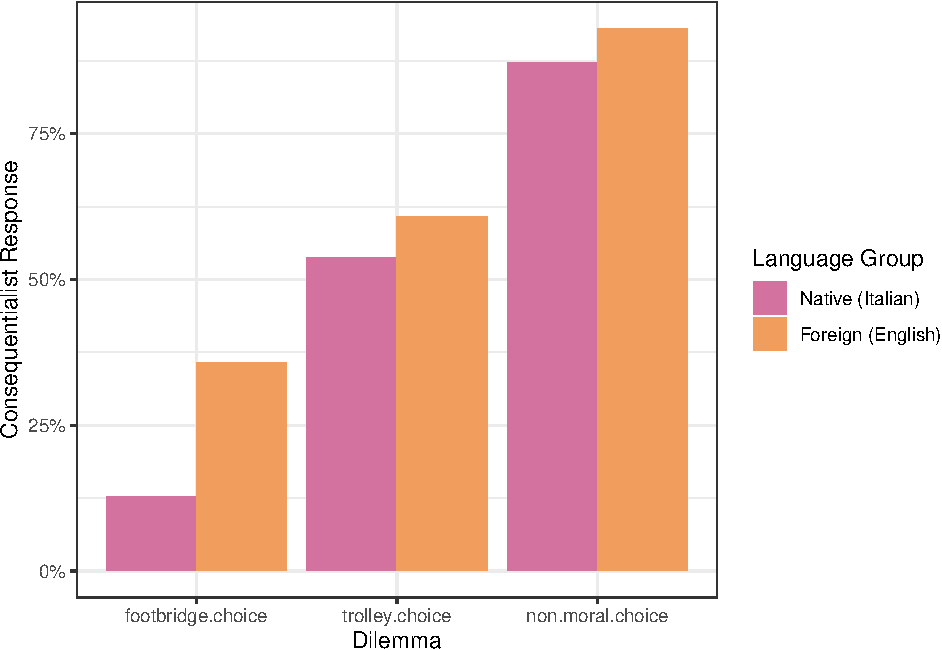
\includegraphics{FLDM_files/figure-latex/English-1.pdf}
\caption{\label{fig:English}Italian versus English}
\end{figure}

\begin{figure}
\centering
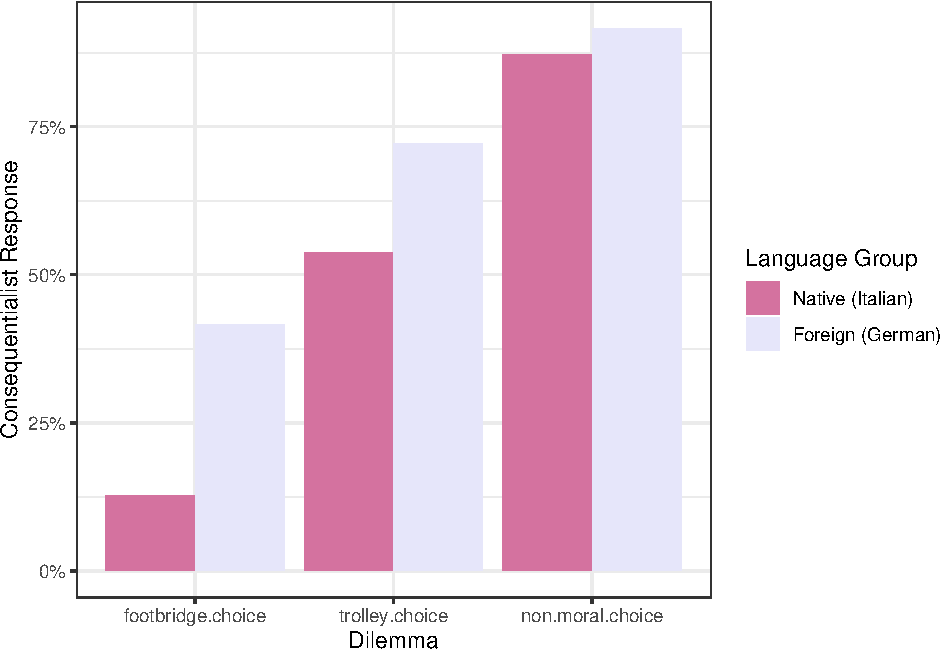
\includegraphics{FLDM_files/figure-latex/German-1.pdf}
\caption{\label{fig:German}Italian versus German}
\end{figure}

\begin{figure}
\centering
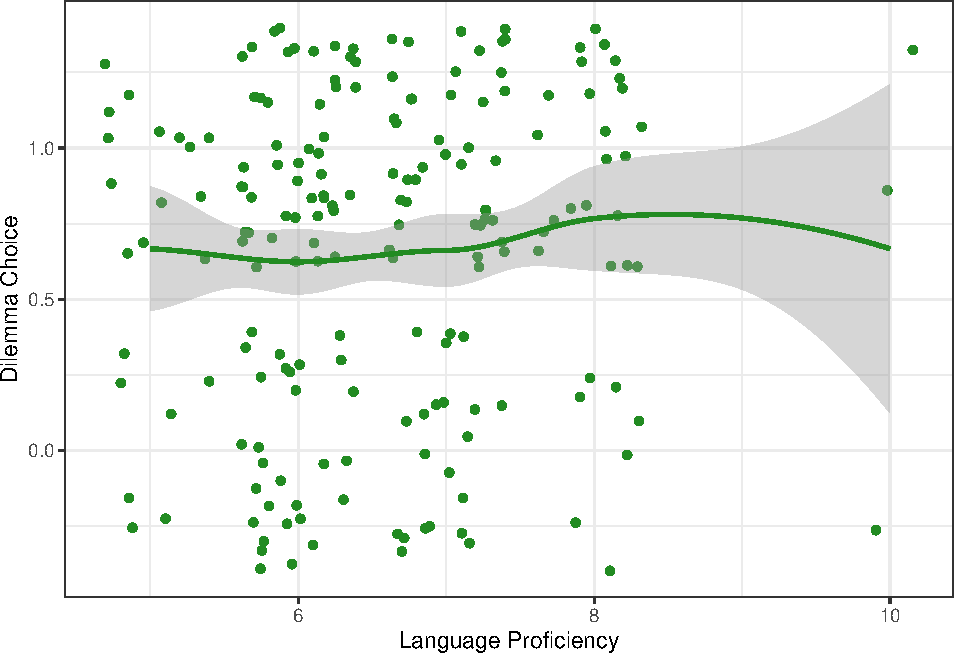
\includegraphics{FLDM_files/figure-latex/Proficiency-1.pdf}
\caption{\label{fig:Proficiency}Proficiency of foreign language.}
\end{figure}

\begin{table}
\centering
\caption{\label{tab:demographic-table}Demographics With Consequentialist Means}
\centering
\begin{tabular}[t]{c|c|c|c|c}
\hline
Condition & N & Trolley Mean \% & Footbridge Mean \% & Non-Moral Mean \%\\
\hline
Italian & 39 & 54\% & 13\% & 87\%\\
\hline
German & 28 & 73\% & 43\% & 92\%\\
\hline
English & 36 & 61\% & 36\% & 93\%\\
\hline
\end{tabular}
\end{table}

\hypertarget{hypothesis-test}{%
\section{hypothesis test}\label{hypothesis-test}}

ANCOVA for effect of language group on dilemma choice for each dilemma type

\hypertarget{results}{%
\section{Results}\label{results}}

A significant effect of dilemma type on consequentialism across language conditions (\(p\) \textless{} .001) is seen showing that any differences in consequentialism are not due to misunderstanding in the foreign language. This is because we expect consequentialism to be highest in the non-moral dilemma (\(\mu\) = 0.90) and lowest in the footbridge dilemma (\(\mu\) = 0.30) . This is because there is no moral dilemma in the non-moral dilemma and therefore no reason to not choose the consequentialist response where as the inverse is true for the footbridge dilemma. The trolley dilemma falls in the middle (\(\mu\) = 0.63). To understand these percentages better, they can be viewed in Figure~\ref{fig:English} and Figure~\ref{fig:German}.

Table~\ref{tab:demographic-table} shows the breakdown of the language categories as well as the mean consequentialism participants exhibited for the different dilemmas. There is a significant effect of
language condition on consequentialism (\(p\) = .017).

\hypertarget{discussion}{%
\section{Discussion}\label{discussion}}

\newpage

\hypertarget{references}{%
\section{References}\label{references}}

\hypertarget{refs}{}
\begin{CSLReferences}{1}{0}
\leavevmode\vadjust pre{\hypertarget{ref-R-papaja}{}}%
Aust, F., \& Barth, M. (2023). \emph{{papaja}: {Prepare} reproducible {APA} journal articles with {R Markdown}}. \url{https://github.com/crsh/papaja}

\leavevmode\vadjust pre{\hypertarget{ref-R-tinylabels}{}}%
Barth, M. (2023). \emph{{tinylabels}: Lightweight variable labels}. \url{https://cran.r-project.org/package=tinylabels}

\leavevmode\vadjust pre{\hypertarget{ref-R-lme4}{}}%
Bates, D., Mächler, M., Bolker, B., \& Walker, S. (2015). Fitting linear mixed-effects models using {lme4}. \emph{Journal of Statistical Software}, \emph{67}(1), 1--48. \url{https://doi.org/10.18637/jss.v067.i01}

\leavevmode\vadjust pre{\hypertarget{ref-R-Matrix}{}}%
Bates, D., Maechler, M., \& Jagan, M. (2024). \emph{Matrix: Sparse and dense matrix classes and methods}. \url{https://CRAN.R-project.org/package=Matrix}

\leavevmode\vadjust pre{\hypertarget{ref-cipollettiMoralForeignLanguageEffect2016}{}}%
Cipolletti, H., McFarlane, S., \& Weissglass, C. (2016). The {Moral Foreign-Language Effect}. \emph{Philosophical Psychology}, \emph{29}(1), 23--40. \url{https://doi.org/10.1080/09515089.2014.993063}

\leavevmode\vadjust pre{\hypertarget{ref-costaYourMoralsDepend2014}{}}%
Costa, A., Foucart, A., Hayakawa, S., Aparici, M., Apesteguia, J., Heafner, J., \& Keysar, B. (2014). Your {Morals Depend} on {Language}. \emph{PLOS ONE}, \emph{9}(4), e94842. \url{https://doi.org/10.1371/journal.pone.0094842}

\leavevmode\vadjust pre{\hypertarget{ref-cummingUnderstandingNewStatistics2013}{}}%
Cumming, G. (2013). \emph{Understanding {The New Statistics}: {Effect Sizes}, {Confidence Intervals}, and {Meta-Analysis}}. {Routledge}.

\leavevmode\vadjust pre{\hypertarget{ref-cushmanRoleConsciousReasoning2006}{}}%
Cushman, F. A., Young, L., \& Hauser, M. (2006). The {Role} of {Conscious Reasoning} and {Intuition} in {Moral Judgment}: {Testing Three Principles} of {Harm}. \emph{Psychological Science}, \emph{17}(12), 1082--1089. \url{https://doi.org/10.1111/j.1467-9280.2006.01834.x}

\leavevmode\vadjust pre{\hypertarget{ref-R-car}{}}%
Fox, J., \& Weisberg, S. (2019). \emph{An {R} companion to applied regression} (Third). Sage. \url{https://socialsciences.mcmaster.ca/jfox/Books/Companion/}

\leavevmode\vadjust pre{\hypertarget{ref-R-carData}{}}%
Fox, J., Weisberg, S., \& Price, B. (2022). \emph{carData: Companion to applied regression data sets}. \url{https://CRAN.R-project.org/package=carData}

\leavevmode\vadjust pre{\hypertarget{ref-geipelForeignLanguageEffect2015}{}}%
Geipel, J., Hadjichristidis, C., \& Surian, L. (2015). The {Foreign Language Effect} on {Moral Judgment}: {The Role} of {Emotions} and {Norms}. \emph{PLOS ONE}, \emph{10}(7), e0131529. \url{https://doi.org/10.1371/journal.pone.0131529}

\leavevmode\vadjust pre{\hypertarget{ref-greenePushingMoralButtons2009}{}}%
Greene, J. D., Cushman, F. A., Stewart, L. E., Lowenberg, K., Nystrom, L. E., \& Cohen, J. D. (2009). Pushing moral buttons: {The} interaction between personal force and intention in moral judgment. \emph{Cognition}, \emph{111}(3), 364--371. \url{https://doi.org/10.1016/j.cognition.2009.02.001}

\leavevmode\vadjust pre{\hypertarget{ref-greeneFMRIInvestigationEmotional2001}{}}%
Greene, J. D., Sommerville, R. B., Nystrom, L. E., Darley, J. M., \& Cohen, J. D. (2001). An {fMRI Investigation} of {Emotional Engagement} in {Moral Judgment} {\textbar} {Science}. \emph{Science}, \emph{293}(5537), 2105--2108. \url{https://doi.org/10.1126/science.1062872}

\leavevmode\vadjust pre{\hypertarget{ref-R-lubridate}{}}%
Grolemund, G., \& Wickham, H. (2011). Dates and times made easy with {lubridate}. \emph{Journal of Statistical Software}, \emph{40}(3), 1--25. \url{https://www.jstatsoft.org/v40/i03/}

\leavevmode\vadjust pre{\hypertarget{ref-hareMoralThinkingIts1981}{}}%
Hare, R. M. (1981). \emph{Moral {Thinking}: {Its Levels}, {Method}, and {Point}}. {Oxford University Press}.

\leavevmode\vadjust pre{\hypertarget{ref-huebnerRoleEmotionMoral2009}{}}%
Huebner, B., Dwyer, S., \& Hauser, M. (2009). The role of emotion in moral psychology. \emph{Trends in Cognitive Sciences}, \emph{13}(1), 1--6. \url{https://doi.org/10.1016/j.tics.2008.09.006}

\leavevmode\vadjust pre{\hypertarget{ref-R-tibble}{}}%
Müller, K., \& Wickham, H. (2023). \emph{Tibble: Simple data frames}. \url{https://CRAN.R-project.org/package=tibble}

\leavevmode\vadjust pre{\hypertarget{ref-R-magick}{}}%
Ooms, J. (2023). \emph{Magick: Advanced graphics and image-processing in r}. \url{https://CRAN.R-project.org/package=magick}

\leavevmode\vadjust pre{\hypertarget{ref-R-base}{}}%
R Core Team. (2023). \emph{R: A language and environment for statistical computing}. R Foundation for Statistical Computing. \url{https://www.R-project.org/}

\leavevmode\vadjust pre{\hypertarget{ref-R-broom}{}}%
Robinson, D., Hayes, A., \& Couch, S. (2023). \emph{Broom: Convert statistical objects into tidy tibbles}. \url{https://CRAN.R-project.org/package=broom}

\leavevmode\vadjust pre{\hypertarget{ref-thomsonTrolleyProblem1985}{}}%
Thomson, J. J. (1985). The {Trolley Problem}. \emph{The Yale Law Journal}, \emph{94}, 1395--1415.

\leavevmode\vadjust pre{\hypertarget{ref-UniTrento}{}}%
{UniTrento}. (n.d.). In \emph{UniTrento}. https://www.unitn.it/en/node/2067.

\leavevmode\vadjust pre{\hypertarget{ref-R-reshape2}{}}%
Wickham, H. (2007). Reshaping data with the {reshape} package. \emph{Journal of Statistical Software}, \emph{21}(12), 1--20. \url{http://www.jstatsoft.org/v21/i12/}

\leavevmode\vadjust pre{\hypertarget{ref-R-ggplot2}{}}%
Wickham, H. (2016). \emph{ggplot2: Elegant graphics for data analysis}. Springer-Verlag New York. \url{https://ggplot2.tidyverse.org}

\leavevmode\vadjust pre{\hypertarget{ref-R-forcats}{}}%
Wickham, H. (2023a). \emph{Forcats: Tools for working with categorical variables (factors)}. \url{https://CRAN.R-project.org/package=forcats}

\leavevmode\vadjust pre{\hypertarget{ref-R-stringr}{}}%
Wickham, H. (2023b). \emph{Stringr: Simple, consistent wrappers for common string operations}. \url{https://CRAN.R-project.org/package=stringr}

\leavevmode\vadjust pre{\hypertarget{ref-R-tidyverse}{}}%
Wickham, H., Averick, M., Bryan, J., Chang, W., McGowan, L. D., François, R., Grolemund, G., Hayes, A., Henry, L., Hester, J., Kuhn, M., Pedersen, T. L., Miller, E., Bache, S. M., Müller, K., Ooms, J., Robinson, D., Seidel, D. P., Spinu, V., \ldots{} Yutani, H. (2019). Welcome to the {tidyverse}. \emph{Journal of Open Source Software}, \emph{4}(43), 1686. \url{https://doi.org/10.21105/joss.01686}

\leavevmode\vadjust pre{\hypertarget{ref-R-dplyr}{}}%
Wickham, H., François, R., Henry, L., Müller, K., \& Vaughan, D. (2023). \emph{Dplyr: A grammar of data manipulation}. \url{https://CRAN.R-project.org/package=dplyr}

\leavevmode\vadjust pre{\hypertarget{ref-R-purrr}{}}%
Wickham, H., \& Henry, L. (2023). \emph{Purrr: Functional programming tools}. \url{https://CRAN.R-project.org/package=purrr}

\leavevmode\vadjust pre{\hypertarget{ref-R-readr}{}}%
Wickham, H., Hester, J., \& Bryan, J. (2023). \emph{Readr: Read rectangular text data}. \url{https://CRAN.R-project.org/package=readr}

\leavevmode\vadjust pre{\hypertarget{ref-R-scales}{}}%
Wickham, H., \& Seidel, D. (2022). \emph{Scales: Scale functions for visualization}. \url{https://CRAN.R-project.org/package=scales}

\leavevmode\vadjust pre{\hypertarget{ref-R-tidyr}{}}%
Wickham, H., Vaughan, D., \& Girlich, M. (2023). \emph{Tidyr: Tidy messy data}. \url{https://CRAN.R-project.org/package=tidyr}

\leavevmode\vadjust pre{\hypertarget{ref-R-psych}{}}%
William Revelle. (2023). \emph{Psych: Procedures for psychological, psychometric, and personality research}. Northwestern University. \url{https://CRAN.R-project.org/package=psych}

\leavevmode\vadjust pre{\hypertarget{ref-R-ggsci}{}}%
Xiao, N. (2023). \emph{Ggsci: Scientific journal and sci-fi themed color palettes for 'ggplot2'}. \url{https://CRAN.R-project.org/package=ggsci}

\leavevmode\vadjust pre{\hypertarget{ref-R-knitr}{}}%
Xie, Y. (2015). \emph{Dynamic documents with {R} and knitr} (2nd ed.). Chapman; Hall/CRC. \url{https://yihui.org/knitr/}

\leavevmode\vadjust pre{\hypertarget{ref-R-kableExtra}{}}%
Zhu, H. (2024). \emph{kableExtra: Construct complex table with 'kable' and pipe syntax}. \url{https://CRAN.R-project.org/package=kableExtra}

\end{CSLReferences}


\end{document}
